\chapter{GUI}

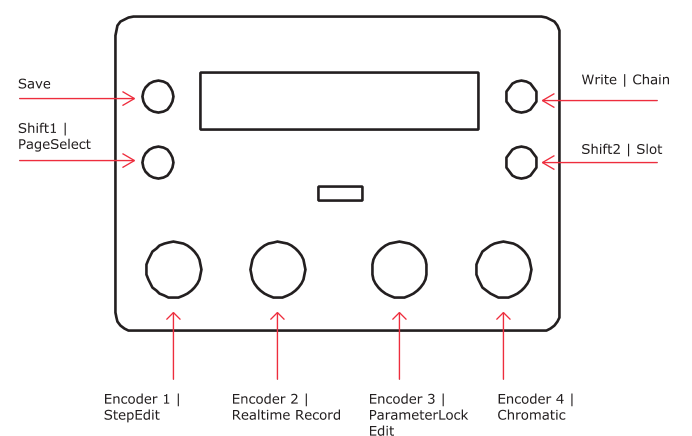
\includegraphics[scale=.6]{mcl_gui.png}\\
The MegaCommand's four upper function buttons are used to enter submenus and activate commands:
\section{Function Buttons:}
From the Grid Page the function buttons perform the following actions:
\begin{itemize}
\item{\textbf{[Save]}: Enters the Save Page}
\item{\textbf{[Write | Chain]}: Enters the Chain page}
\item{\textbf{[Shift1 | PageSelect]}: Enters the PageSelect page}
\item{\textbf{[Shift2 | Slot]}: Opens the slot Menu }
\end{itemize}
Combined Button Presses:
\begin{itemize}
\item{\textbf{[Save] + [ Write | Chain ]}: Opens the Global Settings menu }
\end{itemize}

\section{Encoder Buttons}
From the Grid Page the encoder buttons are used to access Sequencer Pages:
\begin{itemize}
\item{\textbf{[Encoder 1]}: Enter sequencer StepEdit page}
\item{\textbf{[Encoder 2]}: Enter sequencer RealTimeRecord page}
\item{\textbf{[Encoder 3]}: Enter sequencer ParameterLock page}
\item{\textbf{[Encoder 4]}: Enter sequencer Chromatic page}

\end{itemize}


